%% 1 row - OpenSWPC
\begin{figure}[tphb]
  \centering
  \iffalse
  \begin{subfigure}[t]{0.48\textwidth}
    \centering
    \begin{tikzpicture}[scale=1, baseline]
      \begin{customlegend}[legend columns=1,legend style={font=\tiny, column sep=2ex},
          legend entries={Eagle/Intel\textregistered\ Xeon\textregistered\ E5-2697 v3,
            ARM Hi1616,
            Intel\textregistered\ Xeon\textregistered\ Gold 6140,
            AMD Epyc 7551,
            Power8+ S822LC
        }]
        \addlegendimage{mark=otimes,solid}
        \addlegendimage{mark=square,solid}
        \addlegendimage{mark=*,solid}
        \addlegendimage{mark=star,solid}
        \addlegendimage{mark=|,solid}
      \end{customlegend}
    \end{tikzpicture}
  \end{subfigure}\hfill
  \begin{subfigure}[t]{0.48\textwidth}
    \centering
    \begin{tikzpicture}[scale=1, baseline]
      \begin{customlegend}[legend columns=1,legend style={font=\tiny, column sep=2ex},
          legend entries={Execution time ,
            Memory use,
            No. of system file inputs,
            No. of system file outputs
        }]
        \addlegendimage{mark=*,solid}
        \addlegendimage{mark=square,solid}
        \addlegendimage{mark=star,solid}
        \addlegendimage{mark=otimes,solid}
      \end{customlegend}
    \end{tikzpicture}
  \end{subfigure}\bigbreak
  \fi
  \begin{subfigure}[t]{0.48\textwidth}
    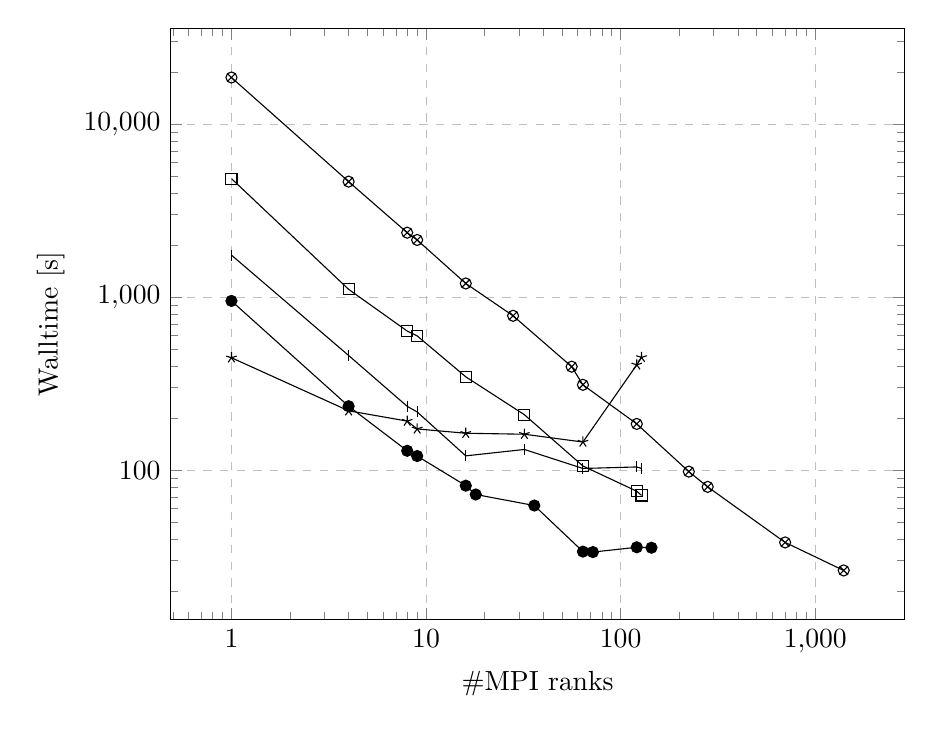
\begin{tikzpicture}[scale=1, baseline]
      \begin{axis}[width=.9\textwidth,height=.75\textwidth,
          xmode=log,
          ymode=log,
          log ticks with fixed point,
          scaled y ticks=real:1e3
          axis lines = left,
          xlabel = \#MPI ranks,
          ylabel = {Walltime [s]},
          %            legend style={at={(0.5,-0.2)},
          %            	    anchor=north,legend columns=1},
          xmajorgrids=true,
          ymajorgrids=true,
          grid style=dashed,
        ]
        %ARM
        \addplot [
          domain=1:150, 
          color=black,
          mark=square,
        ]
        coordinates {
          (1,4840)(4,1109)(8,636.4)(9,596.9)(16,346.1)(32,209.1)(64,105.6)(121,75.5)(128,71.4)
        };
        %                \addlegendentry{ARM Hi1616}
        %Intel 6140
        \addplot [
          domain=1:150, 
          color=black,
          mark=*,
        ]
        coordinates {
          (1,950.4)(4,234)(8,129.3)(9,120.6)(16,81.3)(18,72.3)(36,62.4)(64,33.8)(72,33.6)(121,35.8)(144,35.6)
        };
        %               \addlegendentry{Intel\textregistered\ Xeon\textregistered\ Gold 6140}
        %AMD Epyc
        \addplot [
          domain=1:150, 
          color=black,
          mark=star,
        ]
        coordinates {
          (1,446.1)(4,220.2)(8,192)(9,173)(16,163.3)(32,161.21)(64,145.3)(121,406)(128,448.1)
        };
        %               \addlegendentry{AMD Epyc 7551}
        %Eagle
        \addplot [
          domain=1:1400, 
          color=black,
          mark=otimes,
        ]
        coordinates {                    (1,18584.8)(4,4649.8)(8,2356.4)(9,2139.0)(16,1198.7)(28,779.8)(56,396.2)(64,311.1)(121,184.9)(224,98)(280,80)(700,38.2)(1400,26.3)
        };
        %              \addlegendentry{Eagle/Intel\textregistered\ Xeon\textregistered\ E5-2697 v3}
        %Power
        \addplot [
          domain=1:150, 
          color=black,
          mark=|,
        ]
        coordinates {
          (1,1748.7)(4,459.8)(8,233.7)(9,216.9)(16,120.9)(32,131.6)(64,102.2)(121,104.3)(128,102.2)
        };
        %                \addlegendentry{Power8+ S822LC}
      \end{axis}
    \end{tikzpicture}
    \caption{OpenSWPC scalability}
    \label{fig:openswpc_scalability}
  \end{subfigure}\hfill
  \begin{subfigure}[t]{0.48\textwidth}
    \centering
    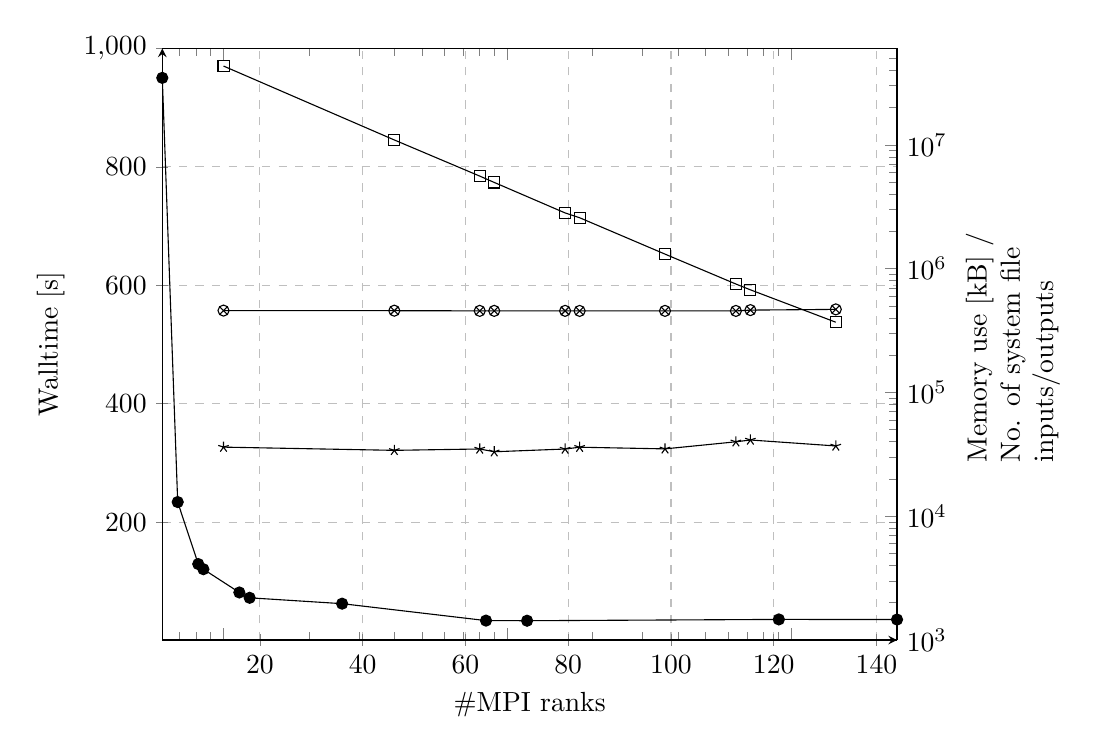
\begin{tikzpicture}[scale=1, baseline]
      \begin{axis}[width=.9\textwidth,height=.75\textwidth,
          %    width=1\textwidth,
          axis y line*=left,
          axis lines = left,
          xlabel = \#MPI ranks,
          ylabel = {Walltime [s]},
          xmajorgrids=true,
          ymajorgrids=true,
          grid style=dashed,
          ymin=1, ymax=1000,
        ]
        %Execution time
        \addplot [
          domain=1:70, 
          color=black,
          mark=*,
        ]
        coordinates {(1,950.4)(4,234)(8,129.3)(9,120.6)(16,81.3)(18,72.3)(36,62.4)(64,33.8)(72,33.6)(121,35.8)(144,35.6)};
        \label{openswpc_execution_time}
      \end{axis}
      \begin{axis}[width=.9\textwidth,height=.75\textwidth,
          xmode=log,
          ymode=log,
          xticklabel=\empty,
          axis y line*=right,
          scaled ticks=false,
          y tick label style={/pgf/number format/.cd,sci,sci e},
          ymin=1000, ymax=60000000,
          ylabel style={text width=3cm},
          ylabel = {Memory use {[kB]} {/} No. of system file inputs/outputs},
          legend style={at={(0.5,-0.2)},
            anchor=north,legend columns=1},
          grid style=dashed,
        ]
        \addlegendimage{/pgfplots/refstyle=openswpc_execution_time}
        %                \addlegendentry{Execution time}
        %RAM
        \addplot [
          domain=1:70, 
          color=black,
          mark=square,
        ]
        coordinates {(1,43267296)(4,10943064)(8,5590132)(9,4967892)(16,2816788)(18,2576328)(36,1309532)(64,751016)(72,674056)(144,368968)};
        %                \addlegendentry{Memory use}
        %#inputs
        \addplot [
          domain=1:70, 
          color=black,
          mark=star,
        ]
        coordinates {(1,36144)(4,34048)(8,34920)(9,33160)(16,34896)(18,36088)(36,34992)(64,39920)(72,41272)(144,36944)};
        %               \addlegendentry{No. of system file inputs}
        %#outputs
        \addplot [
          color=black,
          mark=otimes,
        ]
        coordinates {(1,458040)(4,457256)(8,455752)(9,455664)(16,455688)(18,455248)(36,455544)(64,455168)(72,462144)(144,468512)};
        %                    \addlegendentry{No. of system file outputs}
      \end{axis}
    \end{tikzpicture}
    \caption{OpenSWPC on Intel Xeon Gold 6140}
    \label{fig:openswpc_intel_gold}
  \end{subfigure}\bigbreak
  %      \caption{Results for OpenSWPC}
  %\end{figure}


  %%2 row - CMAQ/CCTM
  %\begin{figure}[ht]
  %\centering
  \begin{subfigure}[t]{0.48\textwidth}
    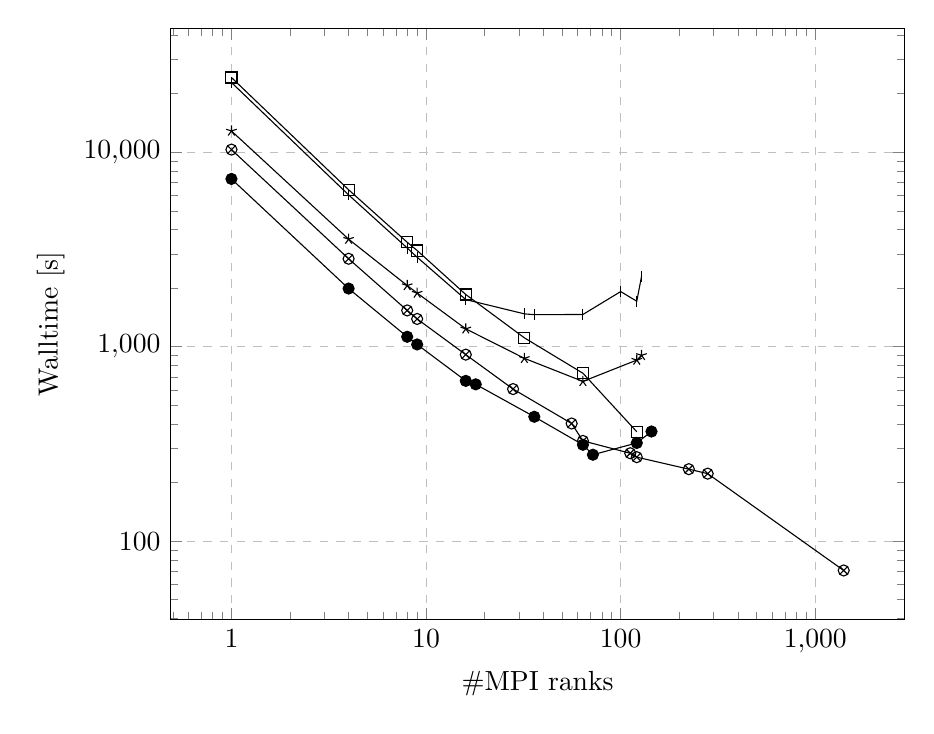
\begin{tikzpicture}[scale=1, baseline]
      \begin{axis}[width=.9\textwidth,height=.75\textwidth,
          %    width=1.3\textwidth,
          xmode=log,
          ymode=log,
          log ticks with fixed point,
          scaled y ticks=real:1e3
          axis lines = left,
          xlabel = \#MPI ranks,
          ylabel = {Walltime [s]},
          %        legend style={at={(0.5,-0.2)},
          %        	    anchor=north,legend columns=1},
          xmajorgrids=true,
          ymajorgrids=true,
          grid style=dashed,
        ]
        %ARM
        \addplot [
          domain=1:150, 
          color=black,
          mark=square,
        ]
        coordinates {
          (1,24239.6)(4,6416.1)(8,3445.6)(9,3124.6)(16,1856.3)(32,1111.4)(64,730.7)(121,365.4)
        };
        %        \addlegendentry{ARM Hi1616}
        %Intel 6140
        \addplot [
          domain=1:150, 
          color=black,
          mark=*,
        ]
        coordinates {
          (1,7294.6)(4,1991.6)(8,1125.1)(9,1027.3)(16,667.5)(18,640.7)(36,436.4)(64,313.2)(72,278.4)(121,320)(144,366.5)
        };
        %        \addlegendentry{Intel\textregistered\ Xeon\textregistered\ Gold 6140}
        %AMD Epyc
        \addplot [
          domain=1:150, 
          color=black,
          mark=star,
        ]
        coordinates {
          (1,12872.6)(4,3574.8)(8,2064.3)(9,1888.6)(16,1235.9)(32,871.8)(64,663.3)(121,853.9)(128,902.9)
        };
        %        \addlegendentry{AMD Epyc 7551}
        %Eagle
        \addplot [
          domain=1:1400,
          color=black,
          mark=otimes,
        ]
        coordinates {
          (1,10323.7)(4,2834.3)(8,1537)(9,1389.7)(16,910.7)(28,605.8)(56,402.9)(64,327.9)(112,283.3)(121,270.5)(224,234.6)(280,222.5)(1400,70.7)
        };
        %       \addlegendentry{Eagle/Intel\textregistered\ Xeon\textregistered\ E5-2697 v3}
        %Power
        \addplot [
          domain=1:150, 
          color=black,
          mark=|,
        ]
        coordinates {
          (1,22849.8)(4,6036.1)(8,3220.3)(9,2885.9)(16,1748.2)(32,1476)(36,1461.4)(64,1465.4)(100,1921.8)(121,1714.5)(128,2297.7)
        };
        %      \addlegendentry{Power8+ S822LC}
      \end{axis}
    \end{tikzpicture}
    \caption{CMAQ/CCTM scalability}
    \label{fig:cmaq_scalability}
  \end{subfigure}\hfill
  \begin{subfigure}[t]{0.48\textwidth}
    \centering
    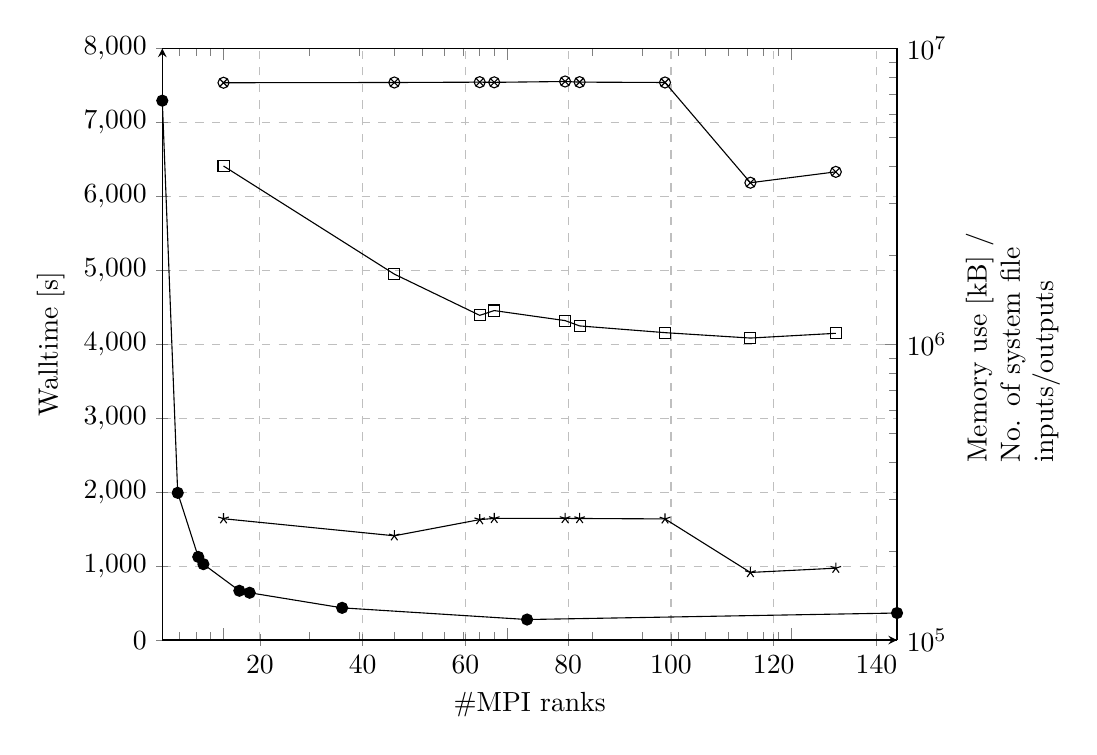
\begin{tikzpicture}[scale=1, baseline]
      \begin{axis}[width=.9\textwidth,height=.75\textwidth,
          %    width=1\textwidth,
          axis y line*=left,
          axis lines = left,
          xlabel = \#MPI ranks,
          ylabel = {Walltime [s]},
          xmajorgrids=true,
          ymajorgrids=true,
          grid style=dashed,
          ymin=1, ymax=8000,
        ]
        %Execution time
        \addplot [
          domain=1:70, 
          color=black,
          mark=*,
        ]
        coordinates {(1,7294.6)(4,1991.4)(8,1125.1)(9,1027.3)(16,667.5)(18,640.7)(36,436.4)(72,278.4)(144,366.5)};
        \label{cmaq_execution_time}
      \end{axis}
      \begin{axis}[width=.9\textwidth,height=.75\textwidth,
          xmode=log,
          ymode=log,
          xticklabel=\empty,
          axis y line*=right,
          scaled ticks=false,
          y tick label style={/pgf/number format/.cd,sci,sci e},
          ymin=100000, ymax=10000000,
          ylabel style={text width=3cm},
          ylabel = {Memory use {[kB]} {/} No. of system file inputs/outputs},
          %                legend style={at={(0.5,-0.2)},
          %                	    anchor=north,legend columns=1},
          grid style=dashed,
        ]
        \addlegendimage{/pgfplots/refstyle=cmaq_execution_time}
        %                \addlegendentry{Execution time}
        %RAM
        \addplot [
          domain=1:70, 
          color=black,
          mark=square,
        ]
        coordinates {(1,4005556)(4,1726776)(8,1252488)(9,1299756)(16,1202224)(18,1153424)(36,1094592)(72,1049436)(144,1089048)};
        %                \addlegendentry{Memory use}
        %#inputs
        \addplot [
          domain=1:70, 
          color=black,
          mark=star,
        ]
        coordinates {(1,257120)(4,225160)(8,255344)(9,257736)(16,257736)(18,257592)(36,256752)(72,169256)(144,174968)};
        %               \addlegendentry{No. of system file inputs}
        %#outputs
        \addplot [
          color=black,
          mark=otimes,
        ]
        coordinates {(1,7660576)(4,7674568)(8,7695080)(9,7684712)(16,7735376)(18,7696800)(36,7676016)(72,3516968)(144,3827848)};
        %                \addlegendentry{No. of system file outputs}
      \end{axis}
    \end{tikzpicture}
    %          \caption{CMAQ/CCTM detailed results for Intel\textregistered\ Xeon\textregistered\ Gold 6140}
    \caption{CMAQ/CCTM on Intel Xeon Gold 6140}
    \label{fig:cmaq_intel_gold}
  \end{subfigure}\bigbreak
  %    \caption{Results for CMAQ/CCTM}


  %%3 row - CM1

  \begin{subfigure}[t]{0.48\textwidth}
    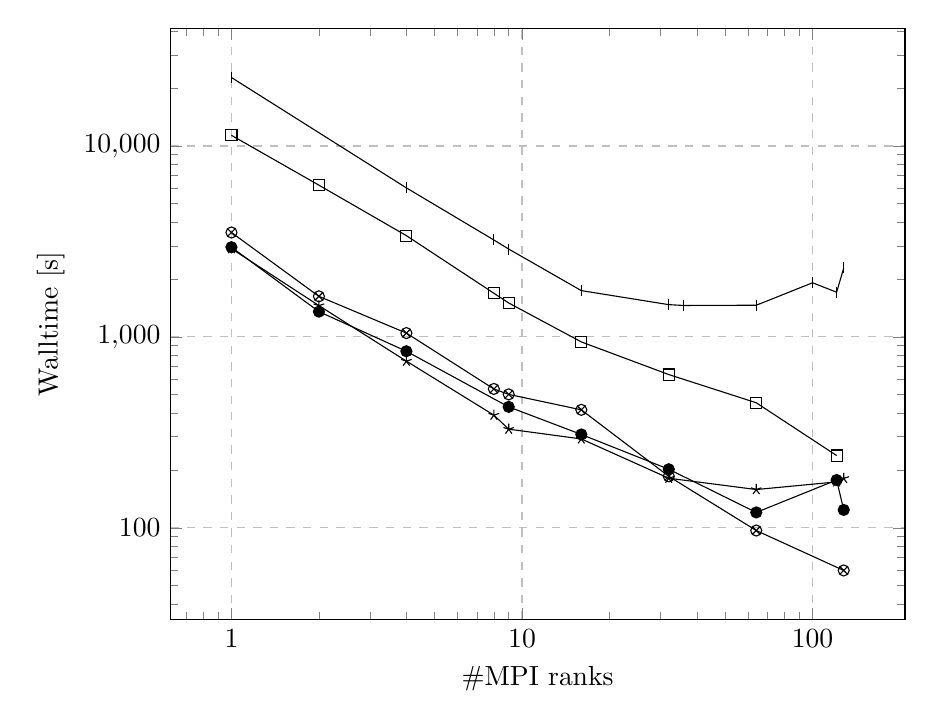
\begin{tikzpicture}[scale=1, baseline]
      \begin{axis}[width=.9\textwidth,height=.75\textwidth,
          xmode=log,
          ymode=log,
          log ticks with fixed point,
          scaled y ticks=real:1e3
          axis lines = left,
          xlabel = \#MPI ranks,
          ylabel = {Walltime [s]},
          %            legend style={at={(0.5,-0.2)},
          %            	    anchor=north,legend columns=1},
          xmajorgrids=true,
          ymajorgrids=true,
          grid style=dashed,
        ]
        %ARM
        \addplot [
          domain=1:150, 
          color=black,
          mark=square,
        ]
        coordinates {
          (1,11379.8)(2,6236)(4,3393.1)(8,1694.1)(9,1505.9)(16,941.5)(32,635.1)(64,452)(121,239.1)
        };
        %           \addlegendentry{ARM Hi1616}
        %Intel 6140
        \addplot [
          domain=1:150, 
          color=black,
          mark=*,
        ]
        coordinates {
          (1,2952)(2,1356.7)(4,841.2)(9,430)(16,308.4)(32,202.7)(64,120.4)(121,178)(128,124.1)
        };
        %          \addlegendentry{Intel\textregistered\ Xeon\textregistered\ Gold 6140}
        %AMD Epyc
        \addplot [
          domain=1:150, 
          color=black,
          mark=star,
        ]
        coordinates {
          (1,2900)(2,1459)(4,746.8)(8,389.4)(9,328.7)(16,292.2)(32,181.9)(64,158.7)(121,174)(128,181.5)
        };
        %            \addlegendentry{AMD Epyc 7551}
        %Eagle
        \addplot [
          domain=1:1400,
          color=black,
          mark=otimes,
        ]
        coordinates {
          (1,3524)(2,1631.4)(4,1047.2)(8,534)(9,500)(16,415)(32,186.1)(64,96.8)(128,59.8)
        };
        %           \addlegendentry{Eagle/Intel\textregistered\ Xeon\textregistered\ E5-2697 v3}
        %Power
        \addplot [
          domain=1:150, 
          color=black,
          mark=|,
        ]
        coordinates {
          (1,22849.8)(4,6036.1)(8,3220.3)(9,2885.9)(16,1748.2)(32,1476)(36,1461.4)(64,1465.4)(100,1921.8)(121,1714.5)(128,2297.7)
        };
        %          \addlegendentry{Power8+ S822LC}
      \end{axis}
    \end{tikzpicture}
    \caption{CM1\ scalability}
    \label{fig:cm1_scalability}
  \end{subfigure}\hfill
  \begin{subfigure}[t]{0.48\textwidth}
    \centering
    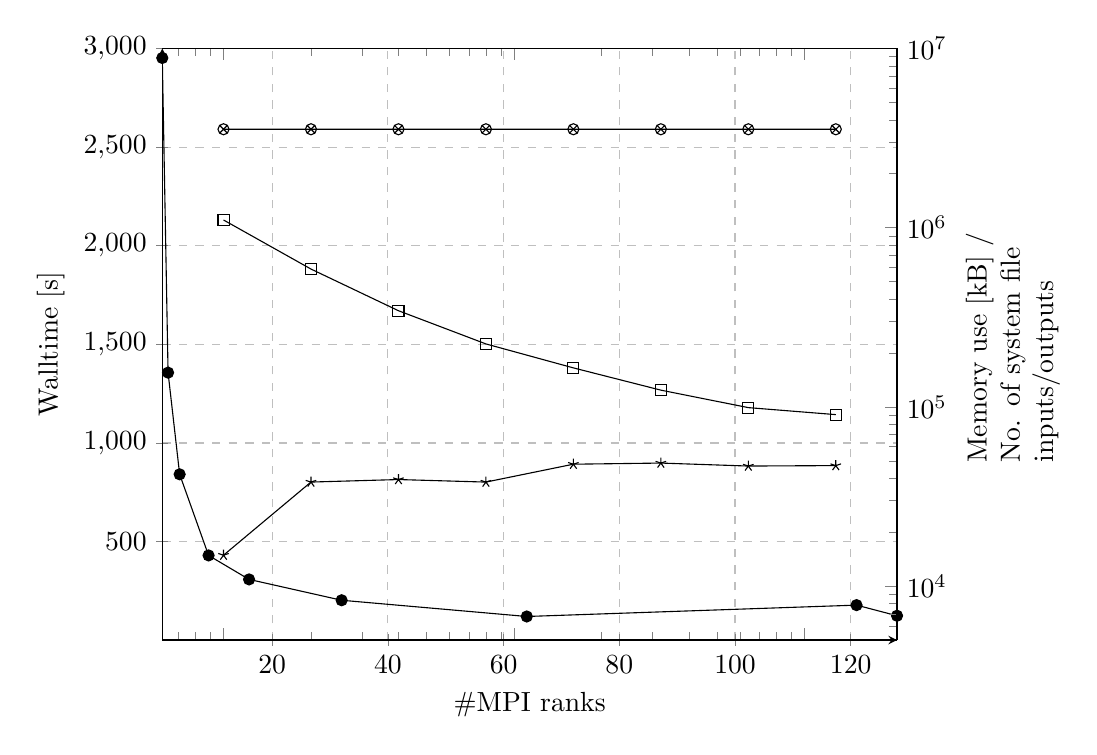
\begin{tikzpicture}[scale=1, baseline]
      \begin{axis}[width=.9\textwidth,height=.75\textwidth,
          %    width=1\textwidth,
          axis y line*=left,
          axis lines = left,
          xlabel = \#MPI ranks,
          ylabel = {Walltime [s]},
          xmajorgrids=true,
          ymajorgrids=true,
          grid style=dashed,
          ymin=1, ymax=3000,
        ]
        %Execution time
        \addplot [
          domain=1:70, 
          color=black,
          mark=*,
        ]
        coordinates {
          (1,2952)(2,1356.7)(4,841.2)(9,430)(16,308.4)(32,202.7)(64,120.4)(121,178)(128,124.1)};
        \label{cm1_execution_time}
      \end{axis}
      \begin{axis}[width=.9\textwidth,height=.75\textwidth,
          xmode=log,
          ymode=log,
          xticklabel=\empty,
          axis y line*=right,
          scaled ticks=false,
          y tick label style={/pgf/number format/.cd,sci,sci e},
          ymin=5000, ymax=10000000,
          ylabel style={text width=3cm},
          ylabel = {Memory use {[kB]} {/} No. of system file inputs/outputs
          },
          legend style={at={(0.5,-0.2)},
            anchor=north,legend columns=1},
          grid style=dashed,
        ]
        \addlegendimage{/pgfplots/refstyle=cm1_execution_time}
        %            \addlegendentry{Execution time}
        %RAM
        \addplot [
          domain=1:70, 
          color=black,
          mark=square,
        ]
        coordinates {(1,1104060)(2,587776)(4,344076)(8,224576)(16,165060)(32,124016)(64,99052)(128,90536)};
        %            \addlegendentry{Memory use}
        %#inputs
        \addplot [
          domain=1:70, 
          color=black,
          mark=star,
        ]
        coordinates {(1,14872)(2,38064)(4,39312)(8,38056)(16,47880)(32,48584)(64,46760)(128,47032)};
        %           \addlegendentry{No. of system file inputs}
        %#outputs
        \addplot [
          color=black,
          mark=otimes,
        ]
        coordinates {(1,3542800)(2,3542536)(4,3542224)(8,3541976)(16,3541912)(32,3541784)(64,3541336)(128,3541336)};
        %            \addlegendentry{No. of system file outputs}
      \end{axis}
    \end{tikzpicture}
    %  \caption{CM1 detailed results for Intel\textregistered\ Xeon\textregistered\ Gold 6140}
    \caption{CM1 on Intel Xeon Gold 6140}
    \label{fig:cm1_intel_gold}
  \end{subfigure}%
  %  \caption{Results for CM1}
  %\end{figure}

  %%4 row - HWRF
  %\begin{figure}[ht]
  \begin{subfigure}[t]{0.48\textwidth}
    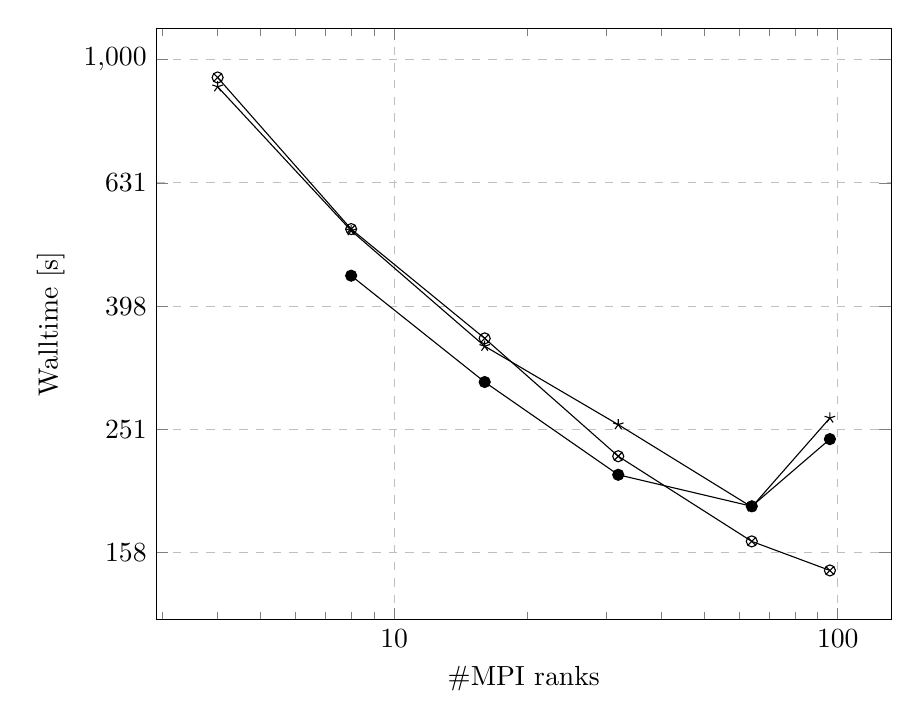
\begin{tikzpicture}[scale=1, baseline]
      \begin{axis}[width=.9\textwidth,height=.75\textwidth,
          xmode=log,
          ymode=log,
          log ticks with fixed point,
          scaled y ticks=real:1e3
          axis lines = left,
          xlabel = \#MPI ranks,
          ylabel = {Walltime [s]},
          %           legend style={at={(0.5,-0.2)},
          %            	    anchor=north,legend columns=1},
          xmajorgrids=true,
          ymajorgrids=true,
          grid style=dashed,
        ]
        %Intel 6140
        \addplot [
          domain=1:150, 
          color=black,
          mark=*,
        ]
        coordinates {(8,446)(16,299.8)(32,212)(64,188.5)(96,242.2)};
        %           \addlegendentry{Intel\textregistered\ Xeon\textregistered\ Gold 6140}
        %AMD Epyc
        \addplot [
          domain=1:150, 
          color=black,
          mark=star,
        ]
        coordinates {
          (4,903.4)(8,527.7)(16,342.7)(32,255.7)(64,188)(96,262.1)
        };
        %          \addlegendentry{AMD Epyc 7551}
        %Eagle
        \addplot [
          domain=1:1400,
          color=black,
          mark=otimes,
        ]
        coordinates {
          (4,935)(8,530.8)(16,352.9)(32,227.2)(64,165.3)(96,148.3)                };
        %          \addlegendentry{Eagle/Intel\textregistered\ Xeon\textregistered\ E5-2697 v3}
      \end{axis}
    \end{tikzpicture}
    \caption{HWRF\ scalability}
    \label{fig:hwrf_scalability}
  \end{subfigure}\hfill
  \begin{subfigure}[t]{0.48\textwidth}
    \centering
    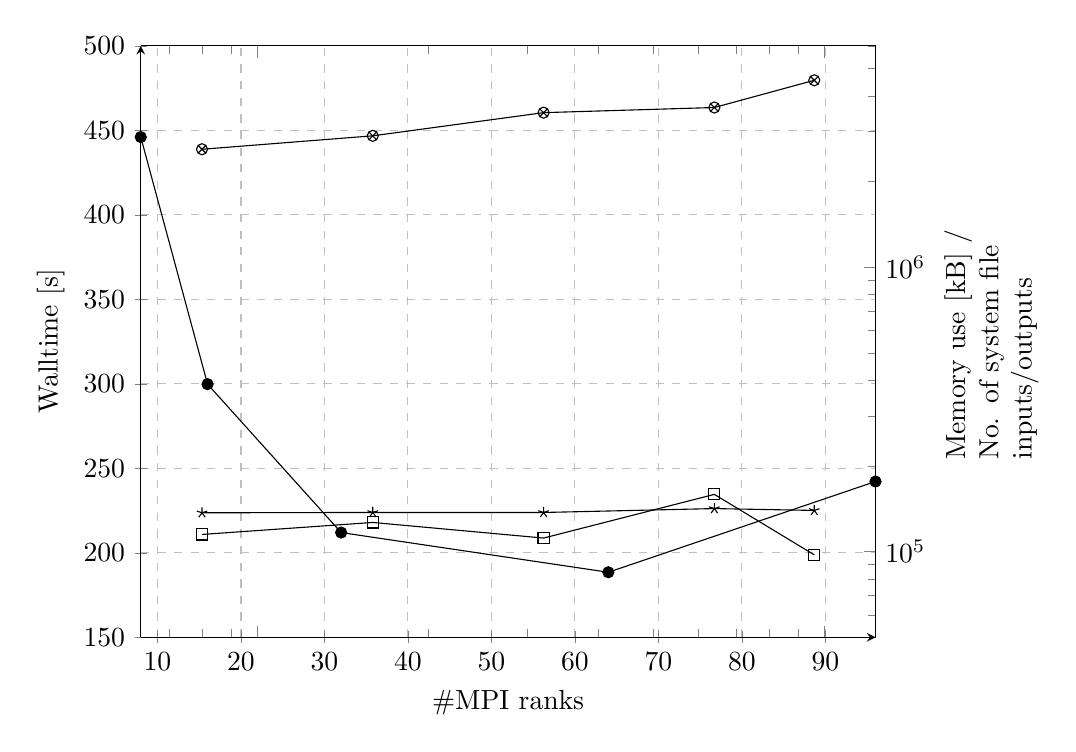
\begin{tikzpicture}[scale=1, baseline]
      \begin{axis}[width=.9\textwidth,height=.75\textwidth,
          axis y line*=left,
          axis lines = left,
          xlabel = \#MPI ranks,
          ylabel = {Walltime [s]},
          xmajorgrids=true,
          ymajorgrids=true,
          grid style=dashed,
          ymin=150, ymax=500,
        ]
        %Execution time
        \addplot [
          domain=1:70, 
          color=black,
          mark=*,
        ]
        coordinates {(8,446)(16,299.8)(32,212)(64,188.5)(96,242.2)};
        \label{hwrf_execution_time}
      \end{axis}
      \begin{axis}[width=.9\textwidth,height=.75\textwidth,
          xmode=log,
          ymode=log,
          xticklabel=\empty,
          axis y line*=right,
          scaled ticks=false,
          y tick label style={/pgf/number format/.cd,sci,sci e},
          ymin=50000, ymax=6000000,
          ylabel style={text width=3cm},
          ylabel = {Memory use {[kB]} {/} No. of system file inputs/outputs
          },
          %            legend style={at={(0.5,-0.2)},
          %            	    anchor=north,legend columns=1},
          grid style=dashed,
        ]
        \addlegendimage{/pgfplots/refstyle=hwrf_execution_time}
        %            \addlegendentry{Execution time}
        %RAM
        \addplot [
          domain=1:70, 
          color=black,
          mark=square,
        ]
        coordinates {(8,114972)(16,126672)(32,111652)(64,158992)(96,97456)};
        %           \addlegendentry{Memory use}
        %#inputs
        \addplot [
          domain=1:70, 
          color=black,
          mark=star,
        ]
        coordinates {(8,136992)(16,137352)(32,137332)(64,141736)(96,139632)};
        %          \addlegendentry{No. of system file inputs}
        %#outputs
        \addplot [
          color=black,
          mark=otimes,
        ]
        coordinates {(8,2596976)(16,2895408)(32,3492632)(64,3641504)(96,4538256)};
        %          \addlegendentry{No. of system file outputs}
      \end{axis}
    \end{tikzpicture}
    \caption{HWRF on Intel\textregistered\ Xeon\textregistered\ Gold 6140}
    \label{fig:hwrf_gold}
  \end{subfigure}\bigbreak
  \caption{Results for CFD applications}
  \label{fig:cfdapps_plots}
\end{figure}

